% vim:ts=4:sw=4
% Copyright (c) 2014 Casper Ti. Vector
% Public domain.

\chapter{系统设计}

\section{匹配算法设计}
在应用上,

对于匹配算法的设计,主要的思想是探究出一种基于用户特征信息来推荐与用户志趣相投的人,所以其中必须要考虑到是现实用户对匹算算法实际效果的满意程度。之后对于不同的意见,对于匹配算法再进行不断对应的调整,从而得到一个相对最优的算法。故此,本文准备采取不同的匹配算法来实验,选取出实验效果最好的来当作最终实施在应用上的算法。同时,该算法可以根据用户的反馈来调整用户的信息的适应性,从而实现程序的自动调节。
\subsection{基于人脸相似度的算法设计}
设变量。。以f当作人脸相似度
 \begin{equation}
   C = \mathop{\argmax}_{c}{\sum_t{w^t_c}}%find how to write down the scripts.
 \end{equation}

\subsection{基于用户信息的算法设计}
根据用户提供的信息,将此当作一个变量添加到匹配算法中,将用户信息提供的信息i设为xi,而对应不同的信息i应该具有不同的匹配算法fi,举个例子,比如年龄信息的可用正态分布的函数对于推荐用户年龄的进行一个匹配,即fi(xi)=正态分布函数。

由此我们可以推导出我们新的匹配算法的公式

但由于用户的兴趣问题,我们针对于用户的猜测可能导致负相关,因此这里的变量越少越好。
\subsection{基于机器学习的算法设计}


\section{face++ SDK for node.js}
由于Face++并没有提供对应的SDK给node.js,所以本研究需要为face++的http请求的api实现一个SDK给node.js。Face++的API如下图
\begin{figure}[h]
\begin{minipage}[t]{0.45\linewidth}
\centering
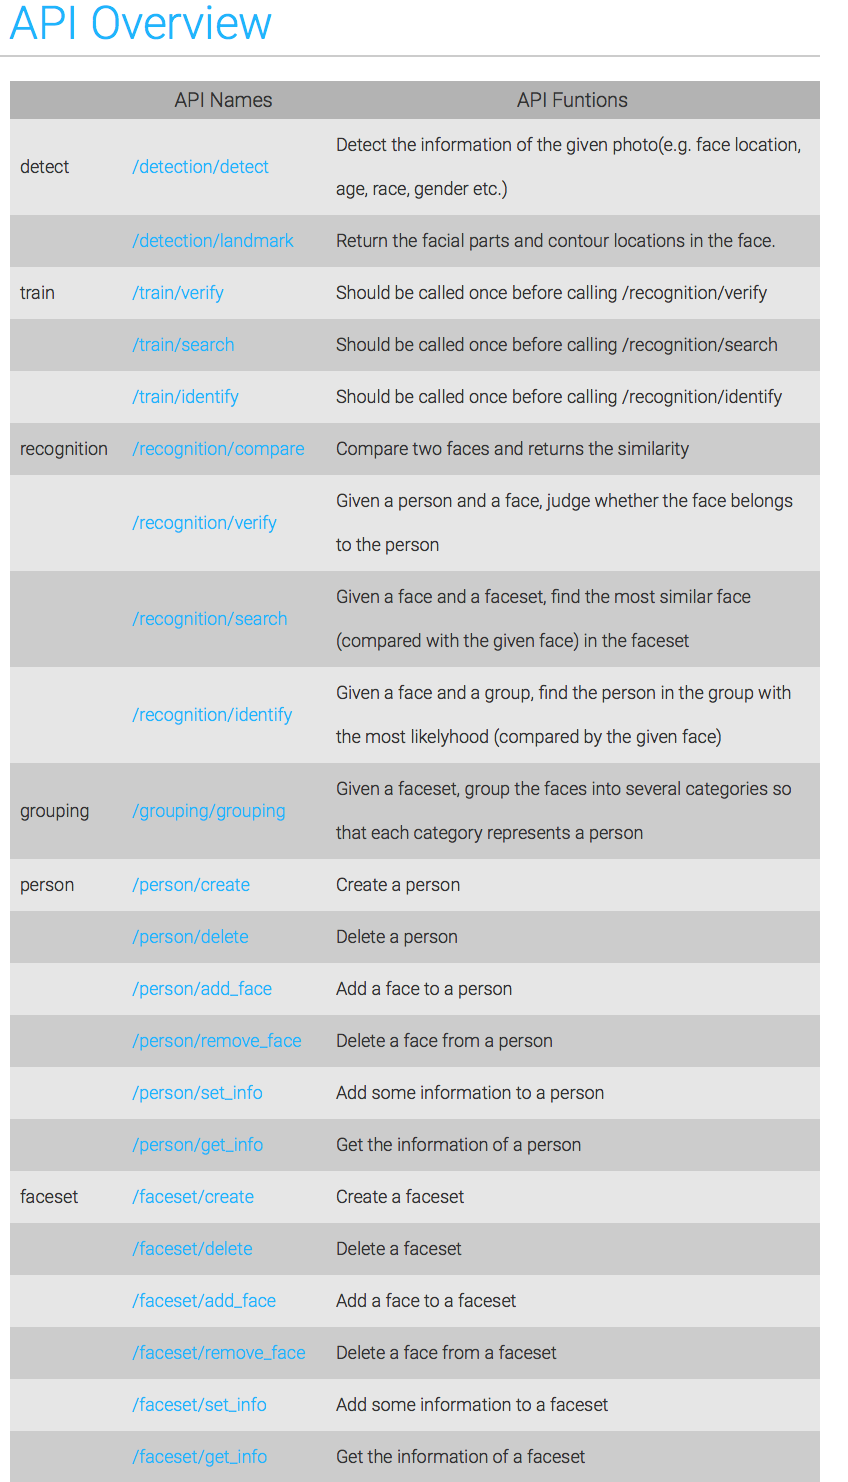
\includegraphics[width=\textwidth]{img/chap2/Face++API.png}
\caption{Face++API\label{Face++API}}
\end{minipage}
\end{figure}


\section{服务器设计}
[用omnigraffle画一个思维导图]


\section{数据库设计}
为了完善我们的数据库的逻辑,本文对于数据库进行了ER图的描述,并用关系行数据库对于NOSQL进行了比对
[用er图]
[用mysql画的一个图]

% 中文测试文字。


